\chapter{System Design}
This chapter will describe the system design of ConnectSphere project, including the frontend and backend architecture, as well as how different components interact to deliver the desired functionality. The frontend of ConnectSphere is developed using React.js, a JavaScript library for building the user interface. The backend of ConnectSphere is built using Node.js and Express.js to provide a reliable server-side environment. This section will present the overview of the frontend and backend architectures. MongoDB was also used to store and retrieve data from the web application.

\section{System Interaction}
The web application works when the frontend interacts with the backend through API requests and responses. When a user creates
or updates a post, the frontend can send an HTTP request to the API endpoint on the backend. The request is processed by the backend. The backend performs the necessary CRUD operations and returns the desired results. The interactions between the  frontend and backend are seamless, allowing for real-time updates and data synchronization throughout the application.

The frontend represents the user interface of the web application, created using technologies such as React and Material-UI. it send HTTP request the backend API to retrieve or manipulate the data. The backend server of ConnectSphere, implemented using Node.js and Express.js. It receives HTTP request from the frontend, performs the necessary operations and return the appropriate response. ConnectSphere uses MongoDB for its flexibility and scalability. MongoDB is where the application's data is stored. The backend interacts with MongoDB to perform the CRUD operations on the data. HTTP requests are made by the frontend to communicate with the backend API. This includes requests to retrieve user data, publish new content, or update user information. After processing the requests and interacting with the database, the backend API return responses with data and status code. The frontend uses this data to update the user interface accordingly. The database operation is performed by the backend API on the database in response to incoming  HTTP requests. Figure 4.1 provides an illustration of the UML diagram. The UML diagram provides an overview of how the various components of ConnectSphere interact with each other to facilitate the flow of data and operation within the application.

\begin{figure}[h!]
    \centering
    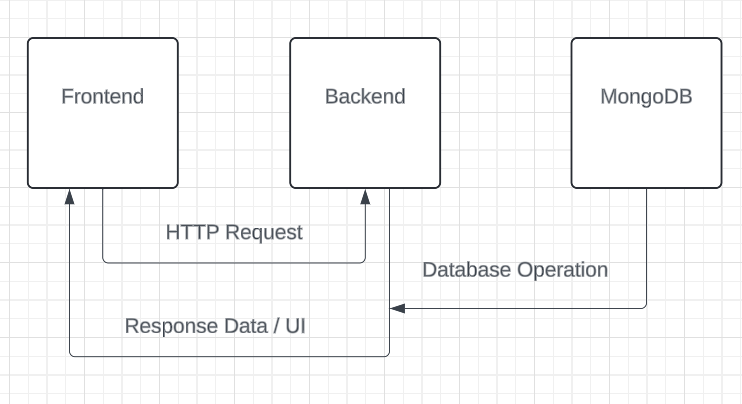
\includegraphics[width=0.7\textwidth]{images/uml.PNG}
    \caption{UML Design}
    \label{fig:uml-design}
\end{figure}



\section{Frontend Architecture}
\subsection{Component-based Structure}
The ConnectSphere uses a component-based structure, with different UI elements are encapsulated within reusable components. This approach enabled the coding process to be flexible and dynamic. Components were combined to build complex user interfaces while keeping the code organized. Each component in the web application serves a specific purpose throughout the application. When creating a post with which users can interact, a component was created to handle all of the post's operations. Another component was designed to display posts, either for the entire application or for a specific user. There is also a component to edit and update a user's post. This allowed the post to be displayed on the home page, where users could interact. Components are imported into other components to extend the application's functionality. The React component-based architecture promotes code reuse effectively. Figure 4.2 depicts the code rendering EditsPostForm component.

\begin{figure}[h!]
    \centering
    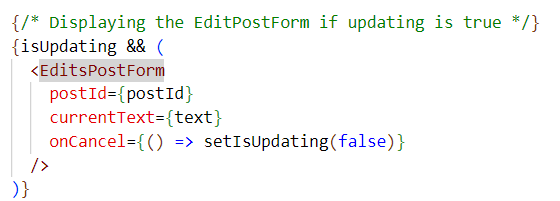
\includegraphics[width=0.7\textwidth]{images/component.PNG}
    \caption{Code snippet from PostWidget.jsx to show EditsPostForm component}
    \label{fig:reusable-component}
\end{figure}

\subsection{Material UI Integration}
Material-UI is a popular React UI framework. Material-UI is integrated into the web application to ensure consistent styling and responsiveness across the social media platform. Material-UI provided numerous pre-built components and styles to help the design of the web application. The design of a social media platform is critical for the project. Material-Ui enabled the application to include important icons for chats, searches and notifications when developing a web application. Material-UI has made ConnectSphere to feel more natural by improving the user interface throughout the application. The social media application can be displayed effectively and simply thanks to the Material-UI tools.

Overall, Material-UI enabled ConnectSphere development to create a visually engaging, responsive, and accessible user interface while maintaining consistency throughout the development process.

\subsection{Redux State Management}
Redux is used to manage the application state, particularly for handling complex state interactions such as user profiles, user authentication, post management and following management. Using Redux state management, the application has a predictable state. The Redux toolkit is used to create slices of state along with their associated reducers. Reducers are defined in each slice that specify how the state should be updated in response to dispatch actions. These slices allow the application to update a user and token in the state when a user sign in or signs out. Specific actions are exported from the slices using destructing, allowing certain parts of the application to import and dispatch these actions. State updating is centralized and consistent across the entire web application.

Actions defined in the slice updates the state immutably. The Redux toolkit handles immutability behind the scenes, allowing for instant state updates without having to worry about modifying the original state object. Redux hooks such as useSelector are used in web application components to access certain parts of states and dispatch actions using useDispatch.

\subsection{API Integration}
The frontend interacts with the backend API endpoints to fetch and update. This allows for communication between the frontend and backend components. Functions are created to handle data fetching operations from the backend API and are typically called when the components are deployed or when certain conditions are met. RESTful API interaction is demonstrated by fetching and handling asynchronous operations using async and wait. Redux actions are dispatched to update the state of the web application with the retrieved data so that it is available to other components. The architecture is designed to follow the best practices for separation of concerns, ensuring that data retrieval logic is isolated from user interface components. Figure 4.3 shows a code snippet for handling comment submissions in a web application.
\begin{figure}[h!]
    \centering
    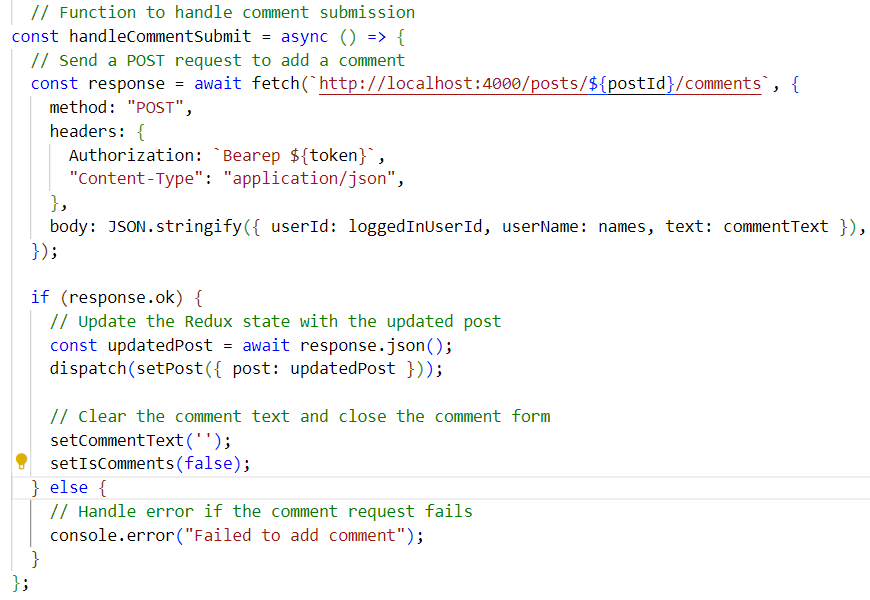
\includegraphics[width=0.9\textwidth]{images/function.PNG}
    \caption{Code snippet from PostWidget.jsx to handle comments}
    \label{fig:comment-function}
\end{figure}

The GET request is used to retrieve the all data from the backend API. The POST, PATCH, and DELETE requests are used in functions to perform various actions, such as liking a post, deleting a post, and adding a reply to a comment. Bearer token is included for authentication, ensuring that only authorized users can perform certain actions like liking post or deleting post. If the response is positive, the Redux state is updated with the updated actions. Error handling is implemented to detect and log any errors that may occur with API requests. Each API interaction is encapsulated in its own function, promoting modularity and code reusability. Socket.IO is used for real-time communication to alert users of certain actions. This improves the user experience by providing instant updates without the need to manually refresh the page. 


\section{Backend Architecture}
\subsection{RESTful API Design}
ConnectSphere follows a RESTful API design pattern where different routes correspond to certain CRUD operations. This allows the application to have a clear and predictable API structure. Making it easier to develop and maintain the backend.
Following RESTful principles for the backend API design ensures a good approach to building scalable and maintainable APIs. Routes are organized around resources such as users and posts, which aligns with RESTful principles. HTTP methods are used to retrieve data, partial updates, delete resources  and create new resources. Parameters are used in the routes to identify certain resources or perform on them.

Error handling is implemented using try-catch blocks in the controller functions to catch errors and send the appropriate HTTP status code along with the error message. This allows the coding process to go smoothly. The error messages pointed to application development issues. The status code indicated whether the error came from the frontend or backend. A middleware function such as 'checkToken' is used to handle the authentication, which is a common practice in RESTful API to ensure security. Security is a crucial aspect of ConnectSphere because it is a social media platform and social networks prioritize security. There is dedicated user search endpoint. This is a best practice to improve API usability.    

\subsection{MongoDB Database}
MongoDB is used as the database for storing user data and post. MongoDB has a flexible schema design that allows you to easily adapt to changing data requirements. Mongoose is an object data modeling library used to communicate with the MongoDB. Mongoose offered a clear approach to defining schemas and performing database operations. MongoDB collections store important data with an unique identifiers for each user document. MongoDB automatically generates the unique identifiers. User collections store information about users and timestamps that indicate when their data was created or updated. Timestamps are managed by MongoDB and are useful for auditing and data analysis purposes. Indexes on the email address field provides uniqueness and optimizes queries for finding users by email address. Mongoose is used to define schemas for the user. The schema applies data validation rules such as required fields, data types, and length restrictions. These data validations ensure the data integrity. Sensitive information, such as passwords, is stored securely using techniques such as password hashing and salting to protect user data from unauthorized access. An array of followers in the user schema to establish a many-to-many relationship between users. Each user document contains an array of user IDs that represent followers. This design allows you to efficiently retrieve a user's followers or find users who follow a specific user. The data types in a user database are shown in the Table 4.1 below.

\begin{table}[ht]
    \centering
    \begin{tabular}{|p{3cm}||p{3cm}||p{5.5cm}|}
    \hline
    \textbf{Field} & \textbf{Datatype} & \textbf{Required} \\
    \hline \hline
    \textunderscore id & ObjectId & Automatically generated \\
    \hline
    userName & String & True \\
    \hline
    emailAddress & String & True \\
    \hline
    password & String & True \\
    \hline
    picturePath & String & False \\
    \hline
    \end{tabular}
        \caption{MongoDB Structure}
         \label{tab:my_label}
\end{table}

\subsection{Authentication Middleware}
JSON web tokens are used for user authentication and authorization. When a successful registration or login occurs, a
JWT token is generated and sent to the client, which is then included in subsequent requests to access secure routes. Middleware functions are used to authenticate the JWT token and grant or restrict access accordingly. Authentication middleware plays a critical role in ensuring that only the authorized users have access to perform certain actions in ConnectSphere. The checkToken middleware function is responsible for verifying JWT tokens sent with incoming requests. The token is extracted from the Permitted header of the HTTP request and if the token is missing, the 403 Forbidden response is returned. The JSON web token library verifies the authenticity of the token using a JWT secret password stored in the environment variable.

When the verification is successful, it attaches the decoded user information with the request object for further processing. When the token verification fails or encounters any error, it returns a 500 internal server error response with the error message. The middleware includes error handling to detect and handle any errors that occur during token processing. If an error occurs, a response is provided with an appropriate HTTP status code to indicating that an error has occurred on the server-side. The middleware helps secure the application. An additional layer of security is added to the application and it is protect against unauthorized access using JWT tokens and their verification with a secret key. The middleware is designed to be reusable across multiple routes and endpoints within the application. This promotes maintainability and scalability of the code by ensuring authentication requirements in different parts of the application without duplicating code.

\section{Application Architecture}
The login system provides users with a secure authentication process to access the application, as shown in Figure 4.4. It offers a user-friendly interface with input fields for email address and password. If the login is successful, users will be redirected to the home page where they can explore ConnectSphere features and content. If users do not already have an account, they can create an account. Users can set up their information such as email, password, profile picture, and username to start exploring the platform. Figure 4.5 depicts the registration page of the application. The homepage serves as the main hub where users explore content, connect with friends, and interact with the community, as shown in Figure 4.6. It provides a personalized feed of posts and activities from users and groups followed by the user, providing engaging and relevant content. Interactive components such as like, dislike and comment buttons allow users to interact with posts and express their opinions. The homepage helps users expand their network by following recommended users. The profile page serves as the user's personal space within the application and displays their identity, interests and activities. Figure 4.7 depicts the profile page. It displays essential information such as the username, profile picture, followers and number of followers and provides a snapshot of the users profile. The profile page displays the user's posts, photos and activities and provides a timeline of their contributions and interactions within the community.

Interactive features such as follow, unfollow buttons and post edit options allow users to connect with others and control their online presence. Integration with chats and notification systems allows users to stay connected, receive updates and have real-time conversations with their friends. The navigation bar provides consistent navigation across different pages of the app, ensuring that users can easily switch between different features and access them without getting lost. The navigation bar provides options related to the user profile, such as viewing notifications, accessing messages and chat functions. The navigation bar adapts the layout and functionality for both desktop and mobile devices. It also includes a search bar that allows users to search for other users within the community.
Overall, the application design focuses on user engagement, personalization and social interaction, providing users with a dynamic and engaging experience to connect. ConnectSphere combines intuitive interfaces, smooth navigation, and interactive features to create meaningful connections between users. The intuitive design, integrated with backend services, contributes to a cohesive and user-friendly experience that allows users to engage with application features.  

\begin{figure}[h!]
    \centering
    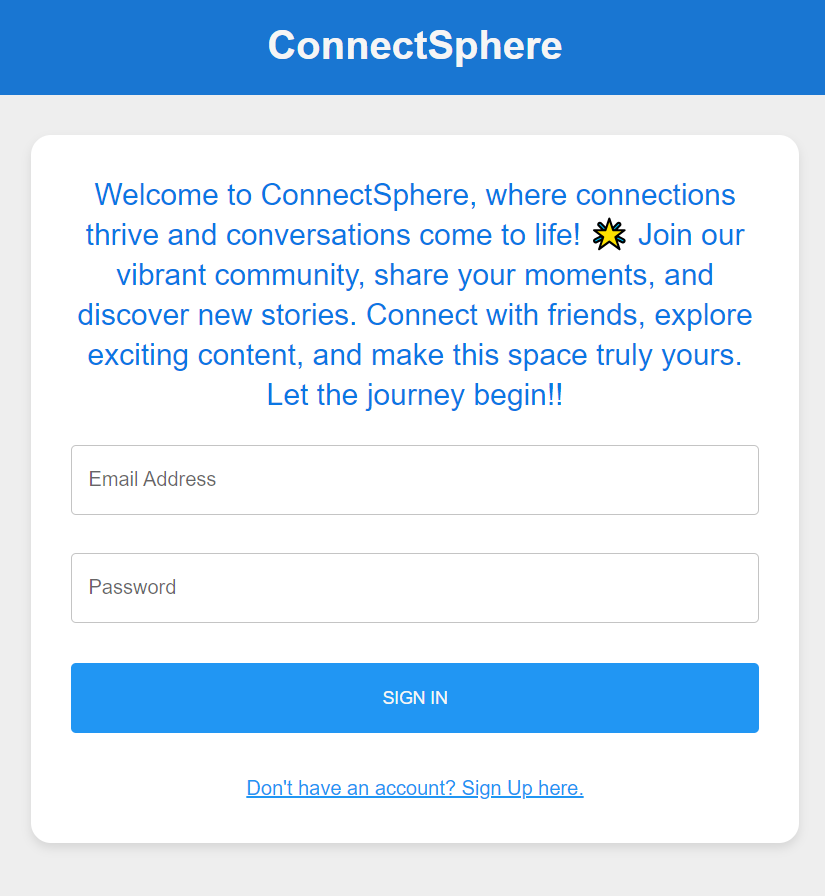
\includegraphics[width=0.7\textwidth]{images/login.PNG}
    \caption{Login Page}
    \label{fig:login}
\end{figure}

\begin{figure}[h!]
    \centering
    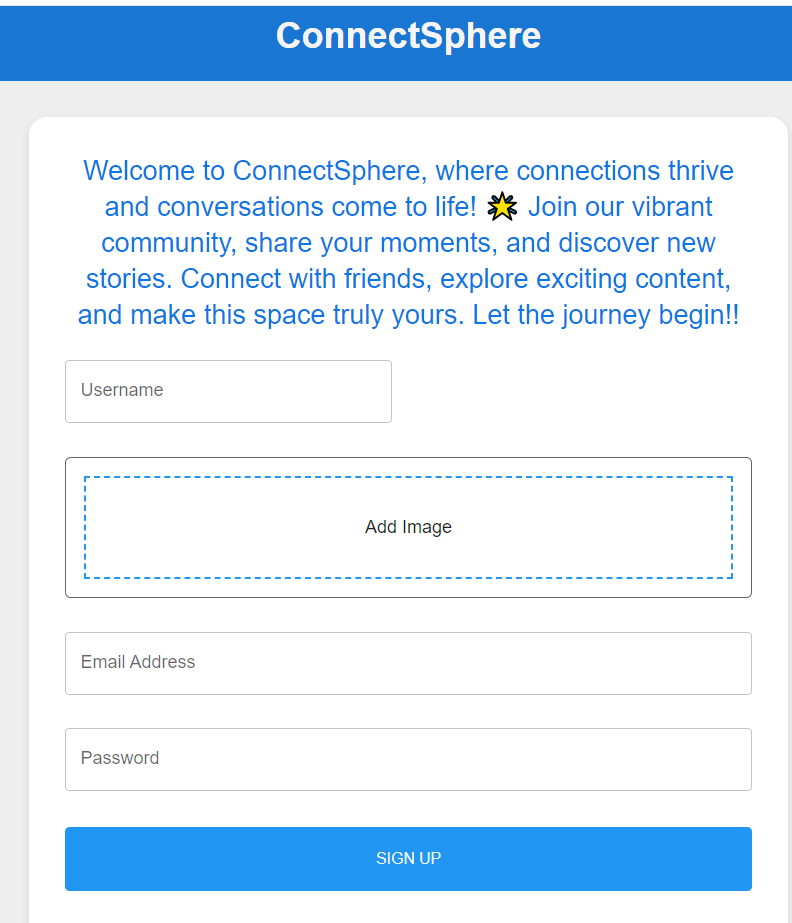
\includegraphics[width=0.7\textwidth]{images/register.PNG}
    \caption{Registration Page}
    \label{fig:register}
\end{figure}

\begin{figure}[h!]
    \centering
    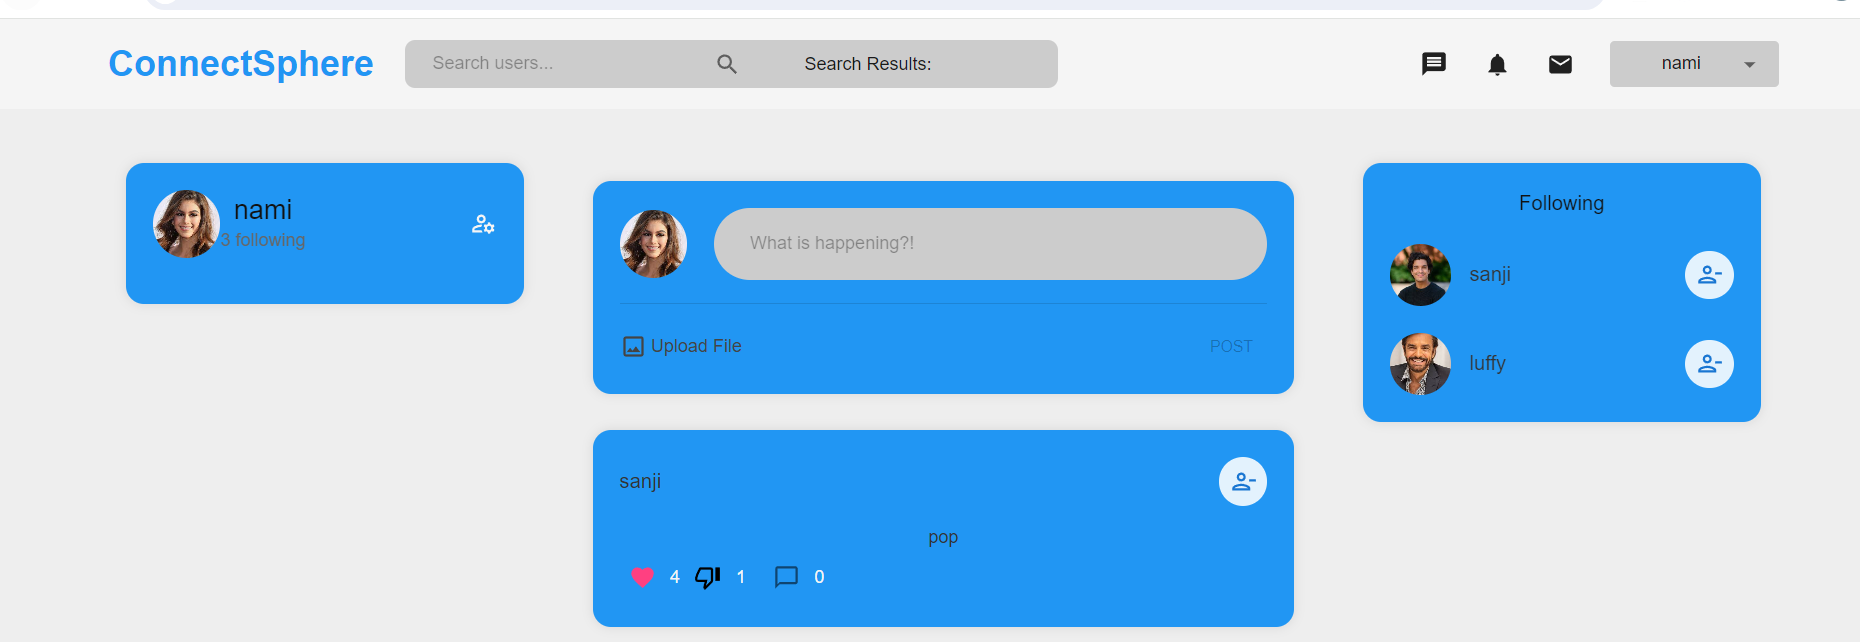
\includegraphics[width=0.7\textwidth]{images/Home.PNG}
    \caption{Home Page}
    \label{fig:home}
\end{figure}

\begin{figure}[h!]
    \centering
    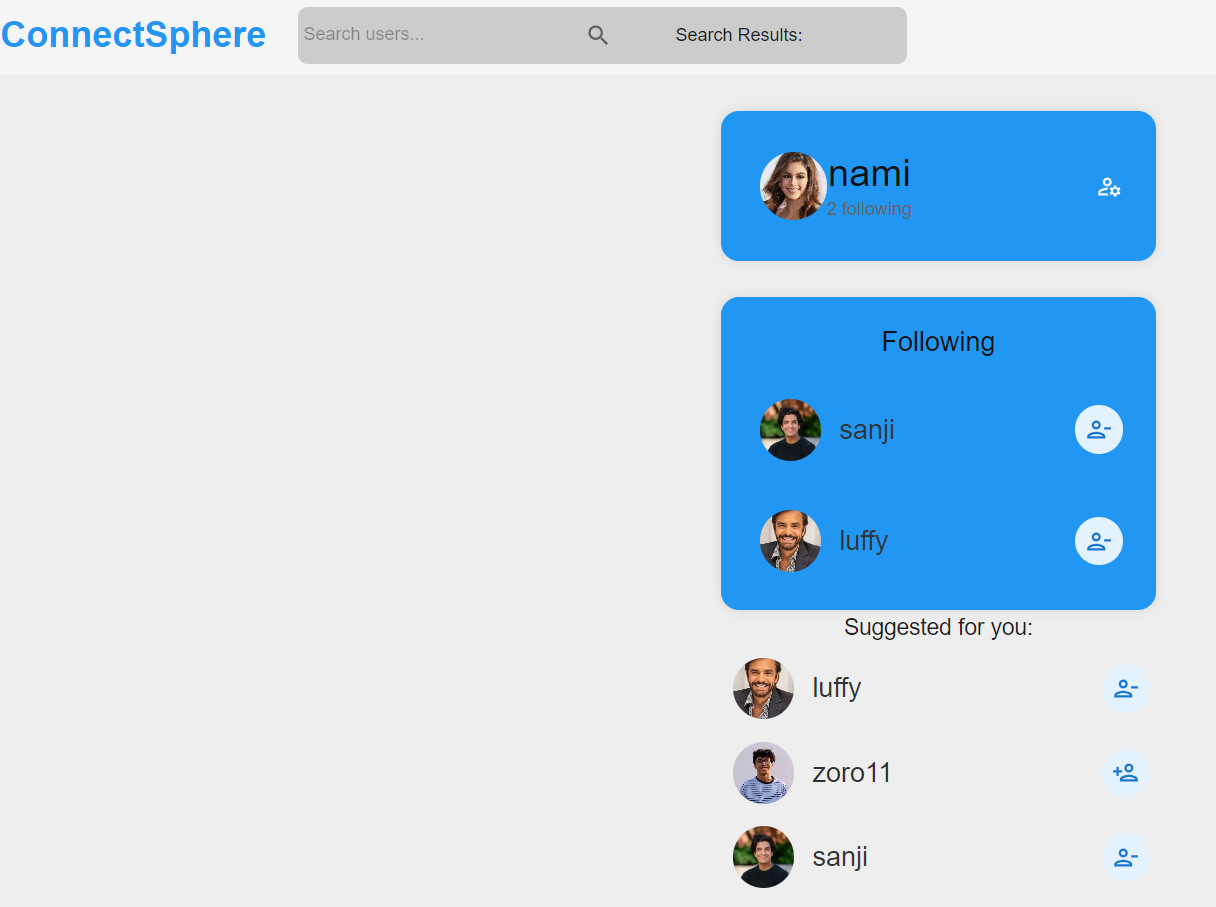
\includegraphics[width=0.7\textwidth]{images/profile.PNG}
    \caption{Profile Page}
    \label{fig:profile}
\end{figure}